% Her skal eg skrive om den nye modellen. Kva er \kappa, kva representerer denne, tid går mot uendelig.. osv.

% Disposisjon:
% 
% 1) kva gir depol. for ein neuron. Kva gir input, kva gir lekkasje?
% 2) utledning av depol.-ligning
% 
%

\section{Mathematical model for the biological neuron}
\label{secMatematiskModelleringAvBioNeuron}
In the biological neuron, the reversal potential for the different ions is can be calculated by the Nernst equation. 
The reversal potential is the potential where opening of the ions channel causes no net current flow through the membrane.

% XXX Skrive inn nernst-equation? Referer kapittel 3 i Bear. (s 65)
\begin{equation}
 	E_{ion} = \frac{C}{z} log\frac{[ion]_o}{[ion]_i}
\end{equation}
Where $E_{ion}$ is the reversal/equilibrium potential for the ion, C is a constant (for some temperature), z is the charge of the ion and $[ion_i]$,$[ion_o]$ gives the number of ions on the inside and outside of the membrane
\cite{NeuroscienceExploringTheBrain3edKAP3}.

For a neuron permeable to a single ion, the equilibrium potential will eventually equal this ions reversal potential. %ref kandel kap 7. s129
For systems where permeability of multiple ions are involved, the equations for each ion becomes a sum of electrical driving force and chemical driving force multiplied with membrane conductance for the ion
\cite{PrinciplesOfNeuralScience4edKAP07}.

At rest, the membrane is a permeable to some ions, and to prevent the ion reaching (and staying) at the membranes equilibrium potential, there are active pumps maintaining a different potential. 
Opening of a membrane channel will change the permeability of the membrane to some ions (depending on the channel), and the ion pumps will not be able to maintain the potential different from the equilibrium potential. 
This is the background for the exitatory and inhibitory postsynaptic potentials (E-PSP/I-PSP)\cite{PrinciplesOfNeuralScience4edKAP07}.
%XXX ref kap 7. kandel. s. 131

Summed up, we have a complex system with continously changing ionic driving force and membrane conductances constantly changing for each ion. 
For artificial neurons used in an ANN most of these aspects can be simplified, and in my system we have one value function giving only the membrane potential. 
The reason behind this is that I do not believe that the individual ions contributions are important enough to justify the extra computational load from the ANN. 
%In addition this is the VANLIGE INNEN SANN.




%Rensa opp litt til hit. *********** fortsett rensing herifra. ****************


%skriv om neste:
The reason for introducing the background information about the neuron is 
\begin{itemize}
	\item to introduce the ide of different states for the neurons membrane. Each with its own equilibrium potential.
	\item to introduce an important consept for the neuron that will be important for ANN as well, $V_{r}$.
	\item to describe the complexity of the system. For a complete simulation of a neuron, each ions distribution across the membrane may need to be simulated as a dynamical system.
	\item to give the background for the system to be modelled as a leaky integrator. The neurons value ``leaks'' toward the equilibrium potential.
\end{itemize}

$V_{r}$ will be used as the resting membranes potential. For biological neurons this can be calculated by the Goldman equation (se \cite{PrinciplesOfNeuralScience4edKAP07}). 
For our use if will be enough to know the extistance of the equilibrium potential for a membrane at rest,
in addition to define a resting membrane potential for the implementation of the artificial neuron.

%For multi--ion systems modelling the system becomes more complicated, but for our use it is enough to know that there is a resting membrane potential that is a function of



%It is important however to know that there is such an equilibrium potential, given by the sum off all the contributions (from the individual ions).

Because of the active pumps, different states with different permeability do the different ions will give different membrane potential because of different factors for each part of the ion differential equation. 
The membrane at rest, that is with no open ion channels, gives the resting membrane potential, $V_r$. 

In the case of synaptic input to a neuron, the postsynaptic membrane will open ligand gated channels (se section \ref{ssecTheNeuron}). 
Both for exitatory and inhibitory input this will push the neurons value and could be seen as an external force in the system.
%For our use, we set this external force to be a constant.
Whether this external driving force can be percieved as a constant or is a more complicated dynamical system is as everything else in the nature; complicated. %Skriv slutten analeis.
The neuron has NMDA channels that are more permeable to both the normal ions in addition to $Ca^{2+}$. Since the NMDA-R is voltage dependent, this causes the glutamatic transmission to be a function of the postsynaptic potential.

%For E input. Kva skjer. Sjå på som eksternt pådrag. 
As this is a mechanism that is little described in articles in neuroscience and to my knowledge not used in ANNs, I will not use voltage dependent exitatory ion channels in my two implementations of ANN. 
%Skriv at dette uansett ikkje har noko innverkning på resultatet? Eller blir dette også dumt i forhold til relevansen til denne linja i teksten?
For my implementations the external driving force on the membrane potential will in other words be a constant.

%Skriv om lekkasje. Forbered på neste seksjon.
%When the potential over the membrane does not equal this equilibrium potential, the system will be driven toward this equilibrium. %(without any external input).

%In the case of neural networks, this is called a 'leaky integrate-and-fire' (LIF) model.

\subsection{The differential equation for neurons depolarization}
The equation for these mechanisms can be stated as a basic differential equation:
\begin{equation}
	\dot{v}(t) = \dot{v}_{in}(I) - \dot{v}_{out}(t), \qquad i = \text{ neural input }
	% skriv også at det er \dot{v}_{out]}(t, v(t)) ---avhengig av v(t) også!
\end{equation}
Where $\dot{v}_{in}(I)$ gives the external input to the neuron (the driving force). % XXX KVA er PÅDRAG på engelsk?
$I$ is the effect of the input to the neuron (sum of exitatory and inhibitory input).

$\dot{v}_{out}(t)$ represents the ``leakage'' of the neurons membrane potential toward the equilibrium potential.


% TODO Ikkje del opp i underavsnitt: Skriv heller "Element for diffligninga", eller noke, og få med begge her.
% Men det eg heller kan ha med som underavsnitt er "forkrav for ligningene" eller "utgangspkt" eller "antagelser for ligningene"...
\subsubsection{The input}
The input, represented by $\dot{v}_{in}(i)$ in the above equation, is a function of the neurons exitatory and inbibitory input. 
The neurons input waries with time, but for now we look at the variable $I$ as a constant in respect to time 
(more on variable input in section \ref{ssecVariableInputBetweenSpikes}).

\begin{equation}
	\dot{v}_{in}(t) = I
\end{equation}
$I$ represents the sum of exitatory and inhibitory input to the neuron.

%skriv også at v_in(i) er i virkeligheita eit dynamisk forløp, men for ANN kan vi forenkle, og sjå på denne som konstant.


\subsubsection{The ``leakage''}
The neuron is often modelled as a leaky integrator. The ``leakage'' is dependent on the polarization over the membrane. 

For biological neurons, the leakage is given as a function of the difference between the membrane potential and the resting membrane potential $V_r$. 
If we define the resting membrane potential for our artificial neuron to be zero, the leakage will vary propotionally to its potential $v(t)$.

%For artificial neurons, we can set this equilibrium potential to zero %for letthetens skuld. Kva blir dette på engelsk?
\begin{equation}
	\dot{v}_{out}(t) = \alpha v(t)
\end{equation}

In a biological neuron, the propotionallity constant, $\alpha$ is given by the distribution of different ion channels active at rest, the extracellular ionic environment compared to the intracellular level of the different ions, etc.
For our basic ANN this will be cept constant. For more advanced versions of this simulator, $\alpha$ could vary as a function of the intracellular ion--levels. 
In addition we have that the extracellular ionic environment is to large extent maintained by glial cells.
%In the CNS you have so--called astricytic domains governed by astrocytes (a certain kind of glial cell). In this domain the 
% BRIFEKUNNSKAP:XXX :  In the CNS you also have socalled astrocytic domains, where the support--cells for the neurons have domains. Inside this domain one astrocyte is 


\subsection{The depolarization equation}%equation for the neurons value}
This gives us the differential equation 
\begin{equation}
	\dot{v}(t) = \dot{v}_{in}(I) - \dot{v}_{out}(t) = I - \alpha v(t)
\end{equation}

Laplace transformation gives
% XXX Legg utledning av uttrykk i appendix! 		Her skal bare stå: V(s) = ...
\begin{equation}
	\begin{split}
		sV(s)-v_0 		&= \frac{I}{s} - \alpha V(s) 			\qquad, \; \qquad v_0 = v(t_0) 				\\
		(s+\alpha)V(s) 	&= \frac{I}{s} + v_0 														\\
		V(s) 			&= \frac{1}{s+\alpha}\left( \frac{I}{s} + v_0 \right)
	\end{split}
\end{equation}

And 
% XXX Legg utledning av uttrykk i appendix! 		Her skal bare stå: V(t) = ...  XXX type: bare siste linja i den kompilerte DVI'en
\begin{equation}
	\begin{split}
		\label{eqVerdiligninga}
		v(t)  	&= 		\mathscr{L}^{-1}\bigg\{ V(s) \bigg\}  									\\
		 		&=		\frac{I}{\alpha} - \frac{I}{\alpha} e^{-\alpha t} + v_0 e^{-\alpha t} 	\\
				&= 		\kappa \left( 1 - e^{-\alpha t} \right) + v_0 e^{-\alpha t} 	\quad,\; \kappa = \frac{I}{\alpha} 
	\end{split}
\end{equation}

Generalization for all neurons is unrealistic due to the divesity of neurons, but for our synthetic neurons we can define that the neuron is reset to the equilibrium potential at rest, $V_r$.
In the simulated neurons this means that after firing, the neuron is reset to $v_0=0$ after firing. 

%If we define a time window as the time interval between time of reset (after firing) to next firing, we can define time $t$ as time after start of time window. This defines the time of reset as $t=0$.
We define the time of reset as $t=0$.

Equation \eqref{eqVerdiligninga} describes a continous nonlinear system. 
In the neuron we have that if the neurons value goes above some threshold the neuron will fire an action potential, and the value is reset. This introduces yet another nonlinearity: 
The action potential.

%\subsection{The inter--spike period}
\subsection{The Action Potential}
Firing of an action potential (a ``spike'') and the period between action potentials (the interspike period) is the basis of the conputational abilities of neurons.
When the value of the neuron excedes the neurons firing threshold an action potential is initialized, and the value is reset to $V_{r}$.

When this is incorporated to the model, this gives that the neuron fires when:
\begin{equation}
	\label{eqTidTilFyringVedEndraKappa}
	\begin{split}
			v(t^*) 					 							&= \tau \qquad 										\\	%,\qquad\qquad\tau = \text{firing threshold} 	\\
			\kappa (1-e^{-\alpha t^*}) + v_0 e^{-\alpha t})		&= \tau 											\\
			(v_0-\kappa)e^{-\alpha t^*}							&= \tau-\kappa 										\\
			\ln \left(e^{-\alpha t^*}\right) 					&= \frac{\kappa - \tau}{\kappa - v_0} 					\\
			t^*													&= -\alpha^{-1} \, \ln \left( \frac{\kappa - \tau}{\kappa - v_0} \right) 					
	\end{split}
\end{equation}

Where $\tau$ is the firing threshold of the neuron. 
If we define $p(\kappa)$ as the inter--spike period (the time from resetting the neuronal value to the next firing)%, $p(\kappa)=t^*$) 
, for constant interspike $\kappa$ we get $v_0 = 0$ and the period given by
\begin{equation}
	\label{eqPeriodeligningForKonstIntraPeriodKAPPA}
	p(\kappa) = -\alpha^{-1} \, \ln(\frac{\kappa - \tau}{\kappa})
\end{equation}

It is impotant to remember that equation \eqref{eqPeriodeligningForKonstIntraPeriodKAPPA} is based on a constant $\kappa$ during the period. 
If $\kappa$ varies during one period, $t^*$ from equation \eqref{eqTidTilFyringVedEndraKappa} is an estimate of the remainting time until firing. This estimate is updated each time $\kappa$ is.



\subsection{Variable input between spikes}
\label{ssecVariableInputBetweenSpikes}
If we assume the input to the neuron to be constant during the interspike period, the equations are simular to the model used in the early ANNs (where the nodes recieves and sends float-values, interpreted as the frequency of the nodes).
% skriv litt annaleis: ikkje "we can read out" men "from eq. ?, the activity can ..." eller noke.
%Given this assumption, we can read out the activity of the neuron from equation \eqref{eqPeriodeligningForKonstIntraPeriodKAPPA}, as the frequency $f(t) = \frac{1}{p(\kappa)}$
Given this assumption, the activity can be read out of eq. \eqref{eqPeriodeligningForKonstIntraPeriodKAPPA} as the frequency $f(t) = \frac{1}{p(\kappa)}$

In this case, the equation is the same as with the frequency based ANNs, with the non-linear activity function of each node based on mechanistic model of the neuron. %MERK: snakk litt om denne `assumption' XXX

%So far we have a non--linear function of the neurons input giving the activity of the neuron. 
%If the activity in the above equation is read out as the freqency ($f(\kappa)=p^{-1}(\kappa)$), 
%the model gets very simular to the traditional frequency based ANN. 
%The non--linear activity function in this model is however based on a mechanistic model of the biological neuron. 

If we allow the input and activity of each neuron to vary between spikes, the model approaches the model for the biological neuron.
%Equation \eqref{eqVerdiligninga} takes into variable leakage as a function of the neurons value %XXX skriv noke slikt som: i motsetning til SANN
For equation \eqref{eqVerdiligninga} to still be valid when $\kappa$ varies within each interspike period, we need to define a time window as the period where $\kappa$ remains constant. 
%Equation \eqref{eqVerdiligninga} can also be used when $\kappa$ varies within each firing period.
%For this we define a time window of $\kappa$ as a time interval where $\kappa$ is constant. 
When $\kappa$ is updated, a new time window will start. 
%$v(t)$ is still defined by equation \eqref{eqVerdiligninga} with $v_0$ given as the value at the start of the time window (the end of the previous time window) and  $t$ representing time into the current time window.
$v_0$ from eq. \eqref{eqVerdiligninga} now represents the value at the start of the time window ( $v_0 = v(t=0)$ ). 
This value is equal to the value $v(t)$ at the time of change from the previous time window(se fig. \ref{figVerdifunskjonen}).
%For eache time window, equation \eqref{eqVerdiligninga} contains the value at the start of the time window ( $v_0 = v(t=0)$ (in the time window) ). 
This is equal to the value of the neuron at the time of variation of $\kappa$ (the value after the previous time window).

In fig. \ref{figVerdifunskjonen}, $v(t)$ is simulated for three different time windows. At time $t_p=100$, $\kappa$ changes from $\kappa_0=0.7$ to $\kappa_1=0.5$. At time $t_p=150$, $\kappa$ becomes $\kappa_2=1$. 
The simulation implies that the value function is a continous function that converges toward the neurons final value, $\kappa$, even for varying $\kappa$.


%\begin{figure}[hbtp]
%	\caption{$v(t)$ for changing $\kappa$. $\kappa_0=0.7$. At time $t_p=100$ $\kappa$ changes to $\kappa_1=0.5$. At time $t_p=150$ the neurons imput increases, and $\kappa_2=1$. See eq.\eqref{eqVerdiligninga}.}
%	\label{figVerdifunskjonen}
%	\begin{center}
%		\includegraphics[width=0.75\textwidth]{demonstrasjonAvUlikeKappaforVerdifunksjonen.ps}
%		%\caption{Demonstration of the value function for changing kappa}
%	\end{center}
%\end{figure}

With this new use of eq. \eqref{eqVerdiligninga}, we can calculate the remaining part of the neurons period after $\kappa$ changes value. 
The remaining time of the period is given by equation \eqref{eqTidTilFyringVedEndraKappa}, given constant $\kappa$. 
If this is updated each time $\kappa$ varies, we get an estimate of the remaining time based on the present $\kappa$.












%********************************************************************************************************************
%********************************************************************************************************************
%*********************     Trur firing cycle skal vekk!  Evt. finn ut korleis det basser inn.  **********************
%********************************************************************************************************************
%********************************************************************************************************************

%mulighet: Kan skrive om det som en måte å visualisere en ide. Sjå for seg en firing cycle, kvar gang $\kappa$ blir oppdatert, regnes \theta ut. Dette gir oss muligheten for å holder oversikt over fase for signalet.
% skriv om firing cycle som eit konsept, tankebane.






%For this we need to introduce a new concept called the firing cycle.

%\subsubsection{The firing cycle}
%(Skriv om firing cycle, men at det er bedre å regne det ut fra verdien fra eq. \eqref{eqVerdiligninga})

%Because of the cyclic nature of the neurons depolarization, it is possible to visualize the neurons interspike period as a firing cycle.
%If we view this as a cycle, the angle $\theta$ can represent the normalized depolarization of the neuron.

%By defining $\omega(\kappa) = \dot{\theta}(\kappa)$ as a function of $\kappa$ over an infinitesimal period of time, the presumption of constant input over the period becomes more realistic. 
%$\kappa$ will then be used to find the derivative of the depolarization of the neuron. For discrete--time systems this infinitesimal period means the least possible time step, one time iteration.

%If we define 
%\begin{equation}
%	\omega(\kappa) = \frac{1}{p(\kappa)}
%\end{equation}

%Since $\omega = \dot{\theta}$, for constant $\kappa$ over some time interval we have that: 
%\begin{equation}
%	\begin{split}
%		\theta^* = \int_0^{t^*} \! \omega(\kappa) \, \mathrm{d}t 		&= 		\int_0^{t^*} \! \frac{1}{ p(\kappa) } \, \mathrm{d}t 	\\
%					\left[\omega(\kappa)\right]_0^{t^*} 				&= 		\left[ \frac{1}{p(\kappa)}\right]_0^{t^*} 				\\
%																	&= 		\frac{t^*}{p(\kappa)}
%	\end{split}
%\end{equation}
%
%We se from this equation that as $t^* = [0,p(\kappa)]$, we have that $\theta=[0,1]$.
%
%Thus $\theta$ represents the normalized depolarization of the neuron. If we for some reason needs to find the depolarization of the neuron this can be calculated by
%\begin{equation}
%	v(t^*) = p(\kappa) \theta^*
%\end{equation}



%If we further introduce the possibility to change $\omega$ an any time during the period, we can sum the contribution of each period with constant $\kappa$:
%%XXX kan vi anta at \theta_0 + \int_0^t \theta dt = \int_{t_0}^t \theta dt ? : JA siden kappa er konstant så varierer ikkje det inne i integralet med integranten (dt)
% 																																									eller ?
%\begin{equation}
%	\begin{split}
%		\theta_{new} = \theta_{old} + \int_{t_0}^{t^*} \! \omega \, \mathrm{d}t 	\qquad \text{stemmer dette?} %	&= 		\int_0^{t^*} \! \frac{1}{ p(\kappa) } \, \mathrm{d}t 	
%	\end{split}
%\end{equation}

%For a discrete--time system the smallest timestep is defined as one time iteration. For such systems we get:
%\begin{equation}
%	\begin{split}
%		\theta^* = \sum_0^{t_n^*} \! \omega  		&= 		\sum_0^{t_n^*} \! \frac{1}{ p(\kappa) } 	\\
%					\left[\omega\right]_0^{t_n^*} 	&= 		\left[ \frac{1}{p(\kappa)}\right]_0^{t_n^*}	\\
%													&= 		\frac{t_n^*}{p(\kappa)}
%	\end{split}
%\end{equation}

%NESTE: Skriv korleis vi kan la input variere når vi gjekk ut fra at input var konstant. 	-- 'Firin cycle'











%kva er forskjellen mellom denne modellen og SANN? Denne modellen holder input fra kvart inputneuron konstant mellom dets spiker(?) mens SANN holder lekkasjen konstant over kvar tidsiterasjon.

